\documentclass[14pt, unknownkeysallowed]{beamer}
\usepackage{tikz}
\usepackage{comment}
\usepackage{fancyvrb}
\usepackage{tikz}
\usetikzlibrary{arrows,decorations.pathmorphing,backgrounds,positioning,fit,petri}
\usepackage{circuitikz} % for circuits!
\usetikzlibrary{arrows.meta} % for loads
\usepackage{float}
\usepackage{listings}

\usepackage{hyperref}

\usepackage[default]{berasans}
\renewcommand*\familydefault{\sfdefault}  %% Only if the base font of the document is to be sans serif
\usepackage[T1]{fontenc}

\setbeamertemplate{navigation symbols}{}
\usetheme{Dresden}
\usecolortheme{seagull}
\usefonttheme{professionalfonts}


\title{Long-Term Simulation of Power System Dynamics using Time Sequenced Power Flows}
\author{Thad Haines}
\institute[MT TECH]{Montana Tech - Master's Thesis Research Project}
\date{February 5th, 2019}

\begin{document}

\begin{frame}
\titlepage
\end{frame}

%************************************************
\section{Introduction}
%________________________________________________
\subsection{Overview of Project}
%------------------------------------------------
\begin{frame}
TODO:\\
What is LTD - why use it \\
system assumptions/main methods of LTD\\
goals of research/ code
\end{frame}
%------------------------------------------------

%************************************************
\section{Simulation Model}
%________________________________________________
%\subsection{Overview of Project}
%------------------------------------------------
\begin{frame}
TODO:\\
Overview of parts involved in simulation (sequence diagram)\\
other explanations about computery stuff: ipy vs py? \\
flow chart of predicted work flow.
\end{frame}
%------------------------------------------------

%************************************************
\section{EE554 System}
%________________________________________________
\subsection{System Used for Initial Frequency Validation}
%------------------------------------------------
\begin{frame}
EE554.sav test system:
\vspace{-1em}\\
\begin{figure}
	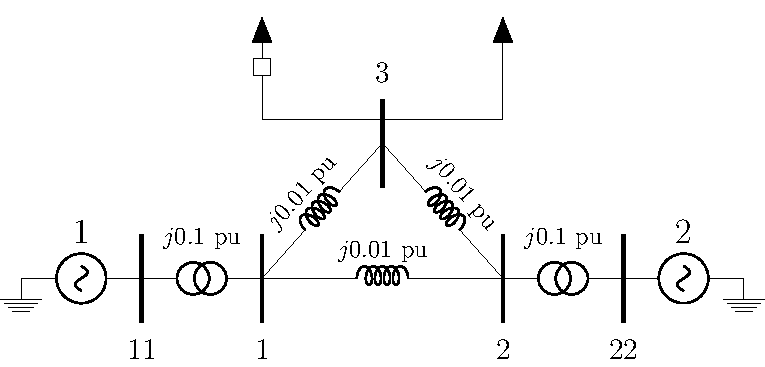
\includegraphics[width=\linewidth]{cicuitEE554}
\end{figure}
\vspace{-1em}
Generators are identical. \\PSLF models have exciters.
\end{frame}
%------------------------------------------------

%************************************************
\section{Validation}
%________________________________________________
\subsection{+20 MW Load Step at t=2}
%------------------------------------------------
\begin{frame}
System Response
\begin{figure}
	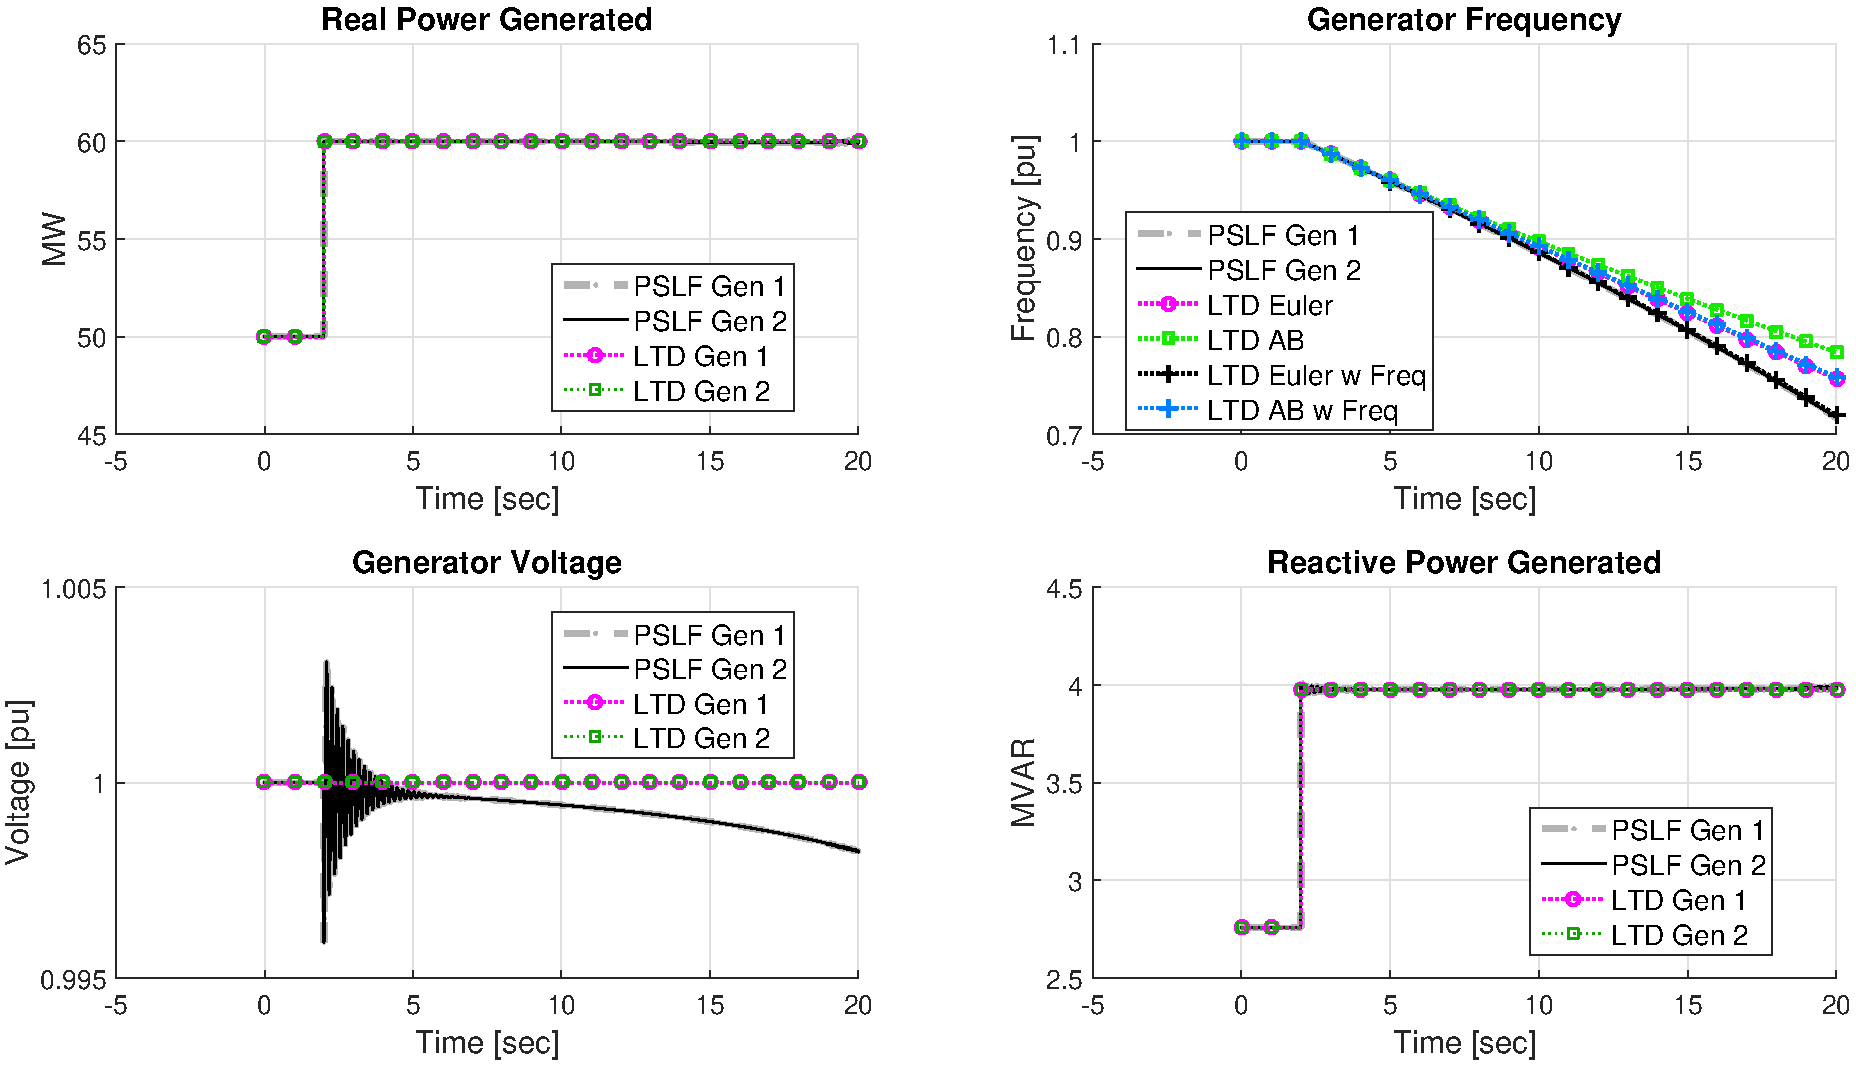
\includegraphics[width=\linewidth]{noGovExcLoadStepUpsys}
\end{figure}
\end{frame}
%------------------------------------------------
\begin{frame}
Detailed Frequency Response
\begin{figure}
	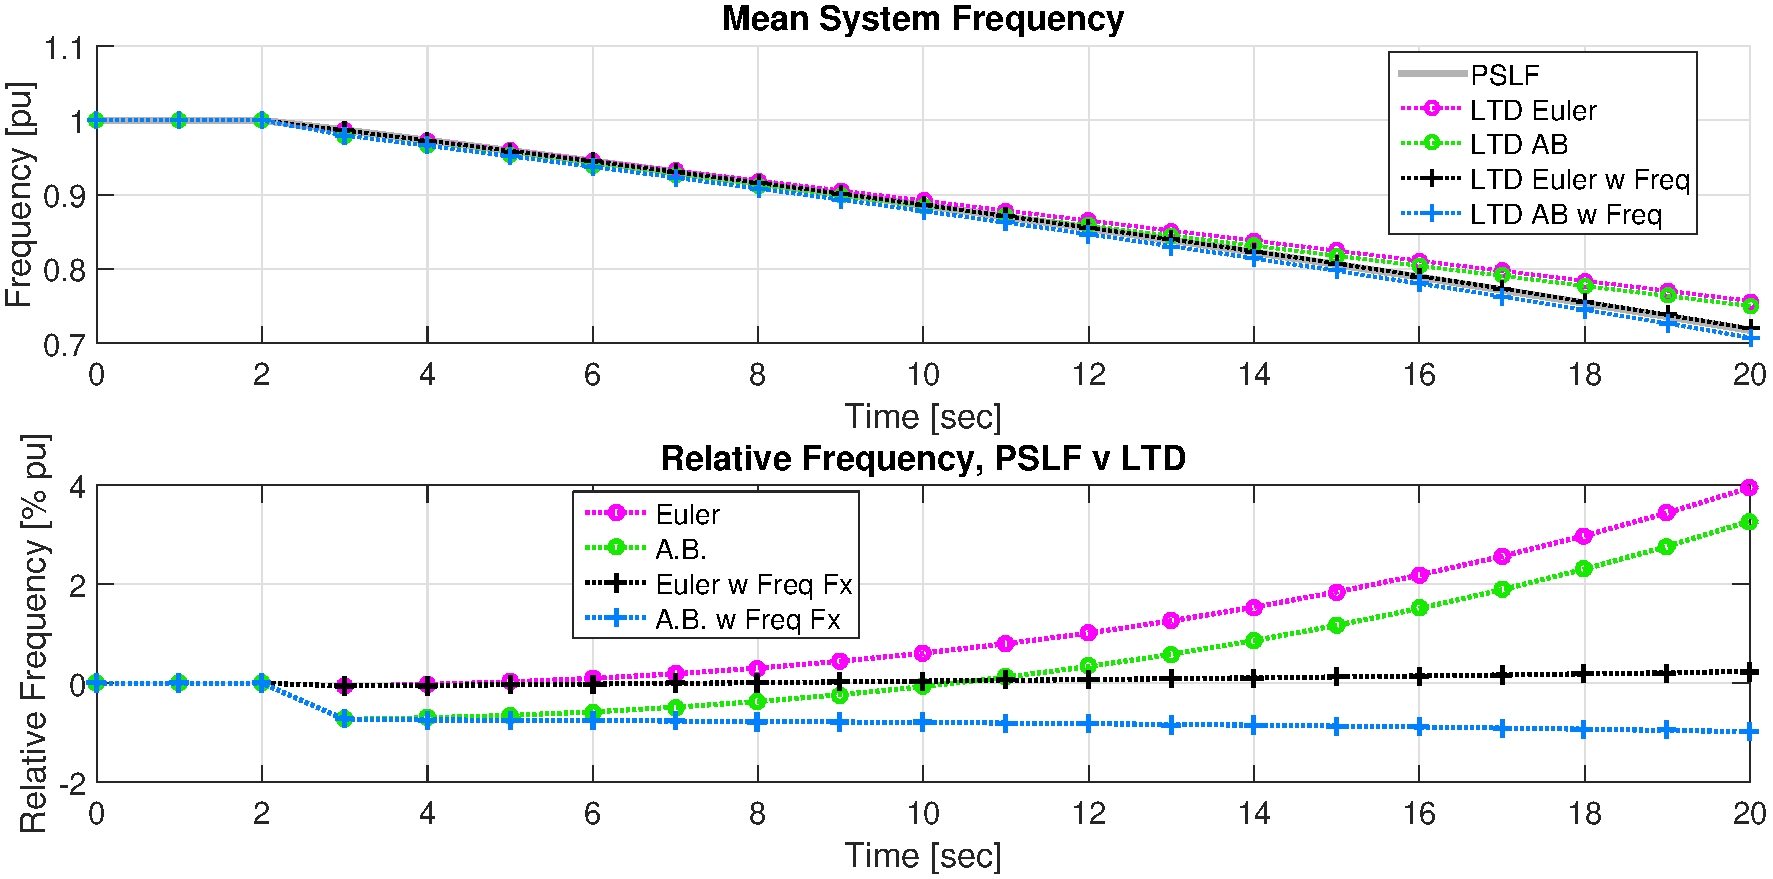
\includegraphics[width=\linewidth]{noGovExcLoadStepUpfreq}
\end{figure}
\end{frame}

%________________________________________________
\subsection{-20 MW Load Step at t=2}
%------------------------------------------------
\begin{frame}
System Response
\begin{figure}
	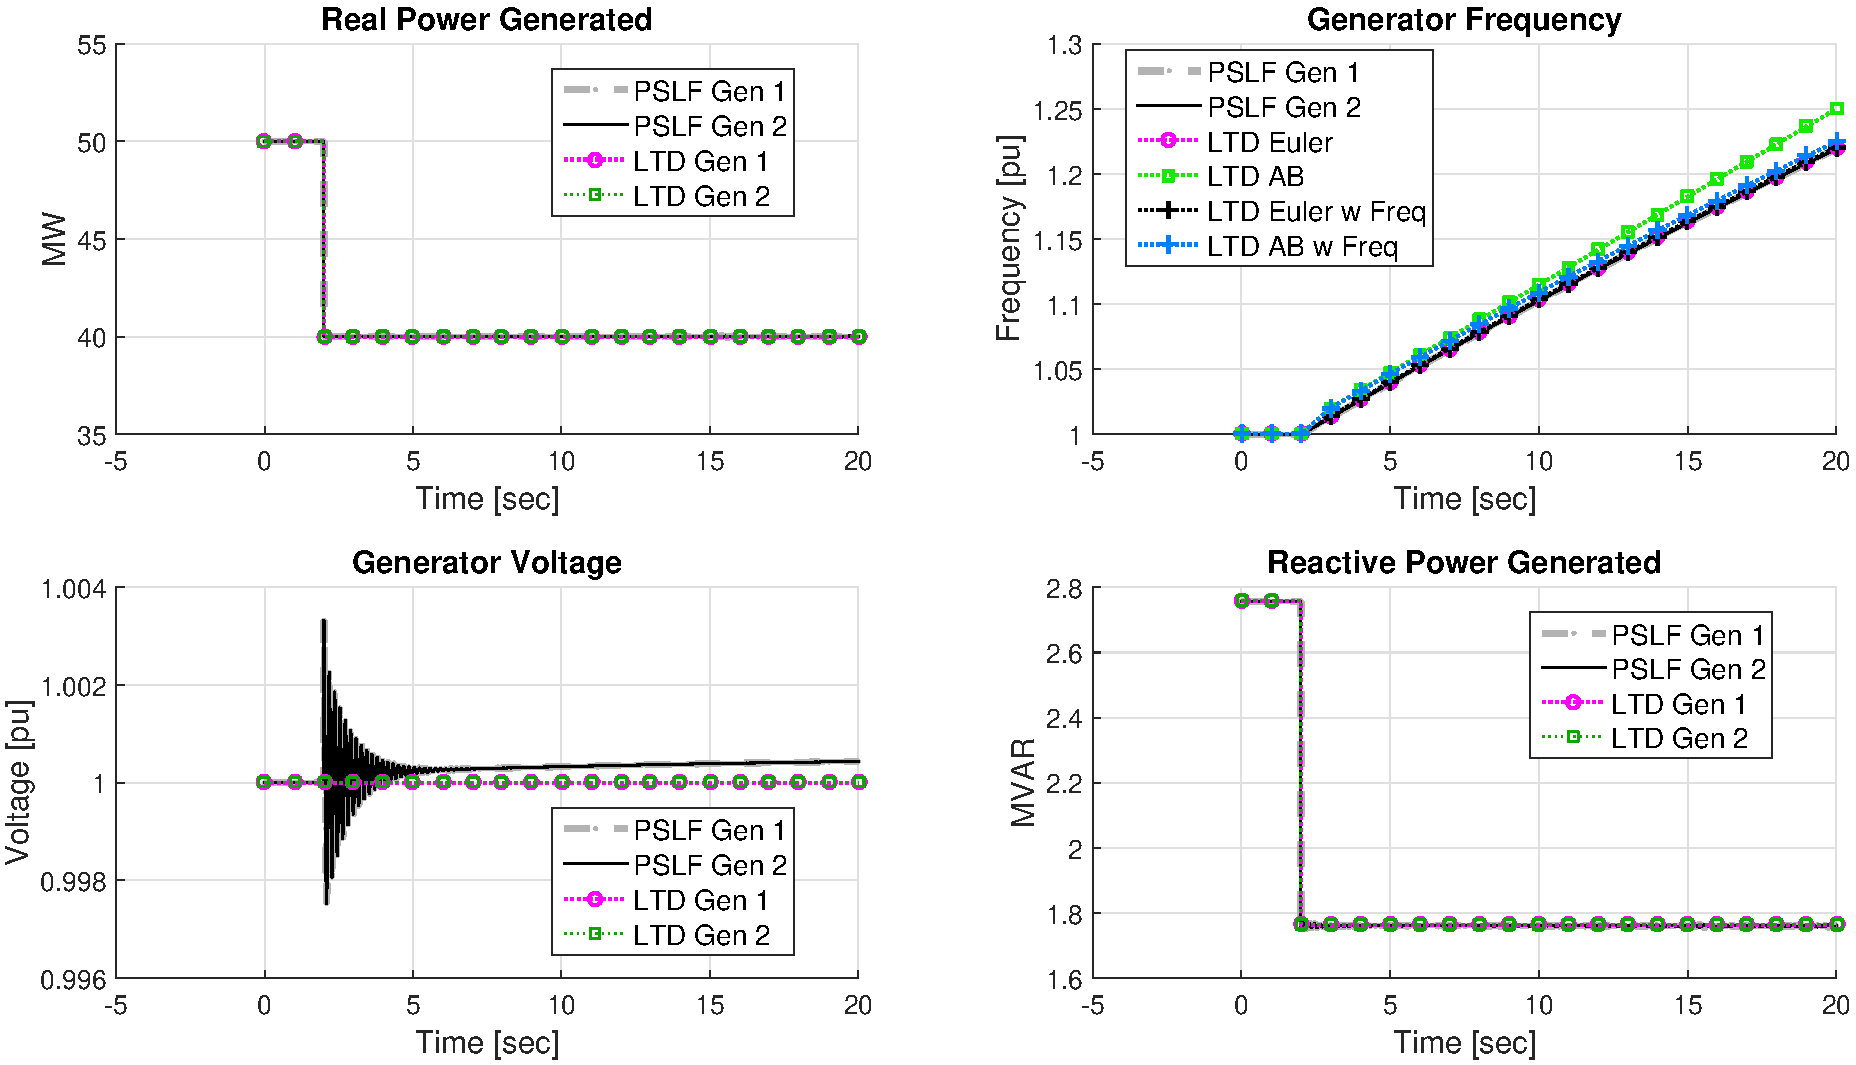
\includegraphics[width=\linewidth]{noGovExcLoadStepDsys}
\end{figure}
\end{frame}
%------------------------------------------------
\begin{frame}
Detailed Frequency Response
\begin{figure}
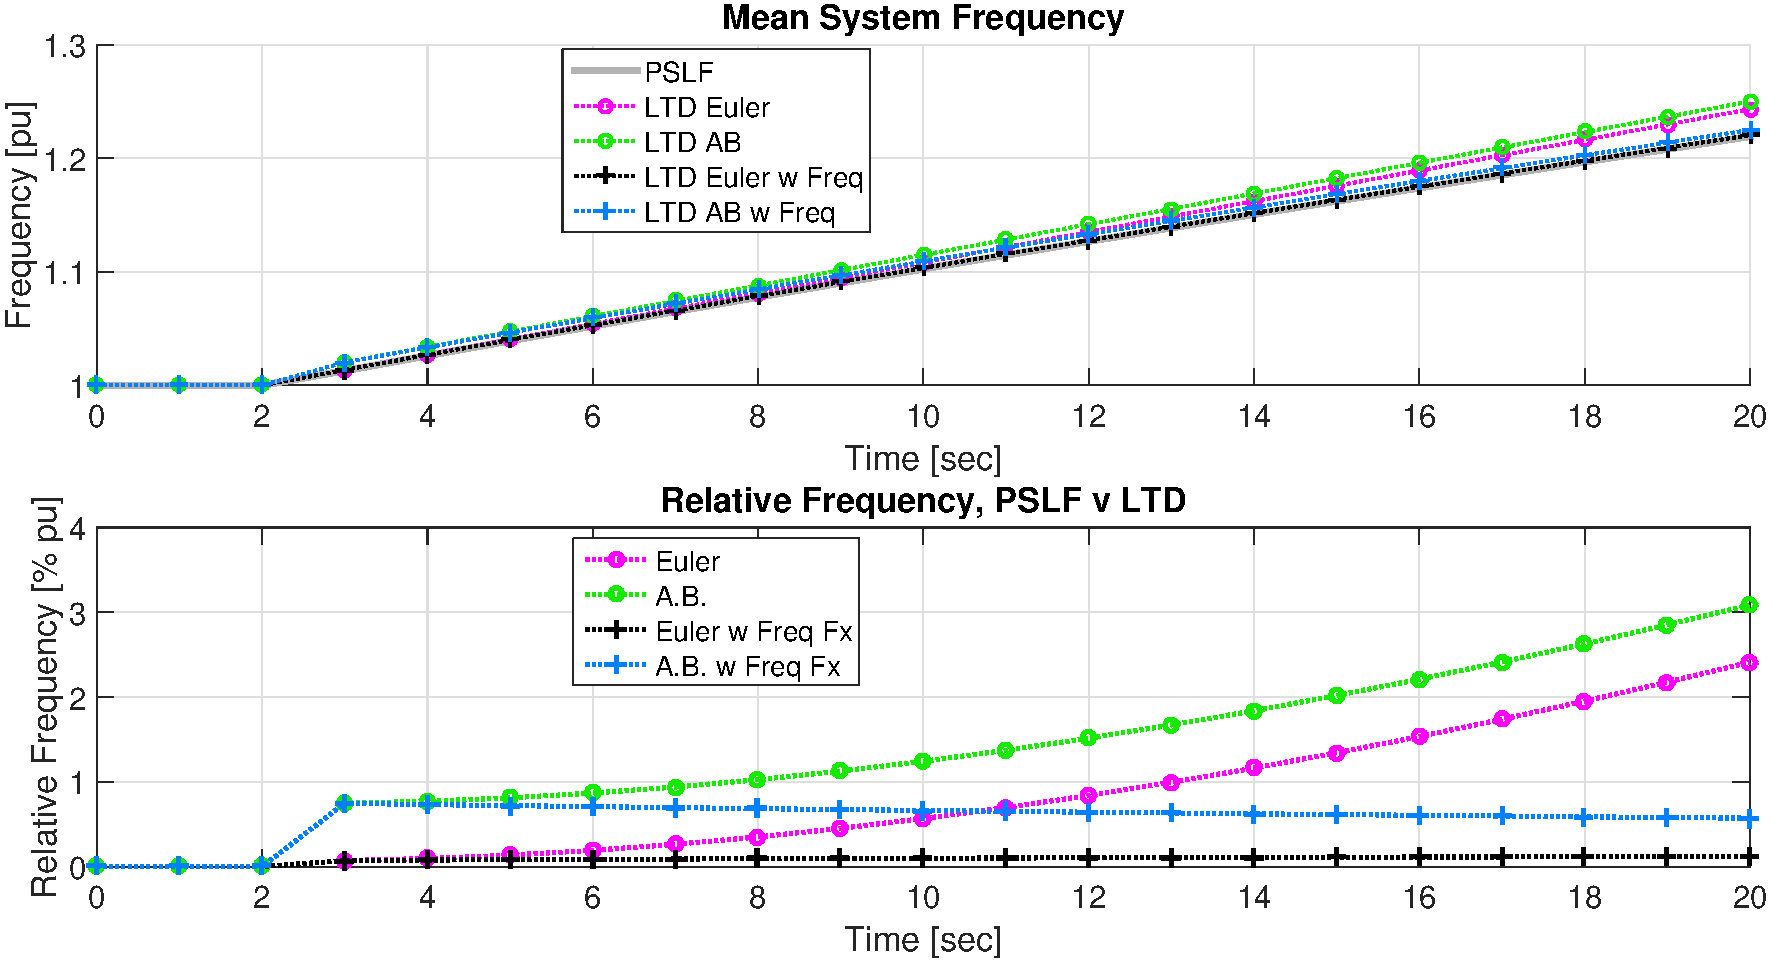
\includegraphics[width=\linewidth]{noGovExcLoadStepDfreq}
\end{figure}
\end{frame}

%************************************************
\section{Proof of Concept}
%________________________________________________
\subsection{Dynamic model 'pgov1'}
%------------------------------------------------
\begin{frame}[fragile]
Proportional gain control of generator $P_M$ 
\begin{figure}
	% this may not be the system we really want... maybe no sbase and k1
	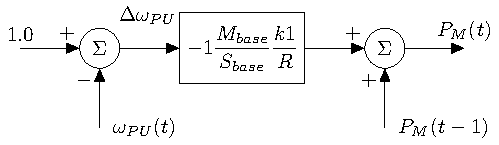
\includegraphics[width=\linewidth]{pgov1}
\end{figure}
Entered into system via parsed text file:
\begin{lstlisting}[basicstyle=\footnotesize]
# pgov1  busnum busnam basekv id : #9 mwcap droop k1
#!pgov1   21 "21" 22.00 "1 " : #9 mwcap=100.0 0.05 13.0
\end{lstlisting}
\end{frame}

%________________________________________________
\subsection{Dynamic model 'pgov1' experiment: -20 MW t=2, +30 MW t=32}
%------------------------------------------------
\begin{frame}
pgov1 on Gen 1
\begin{figure}
	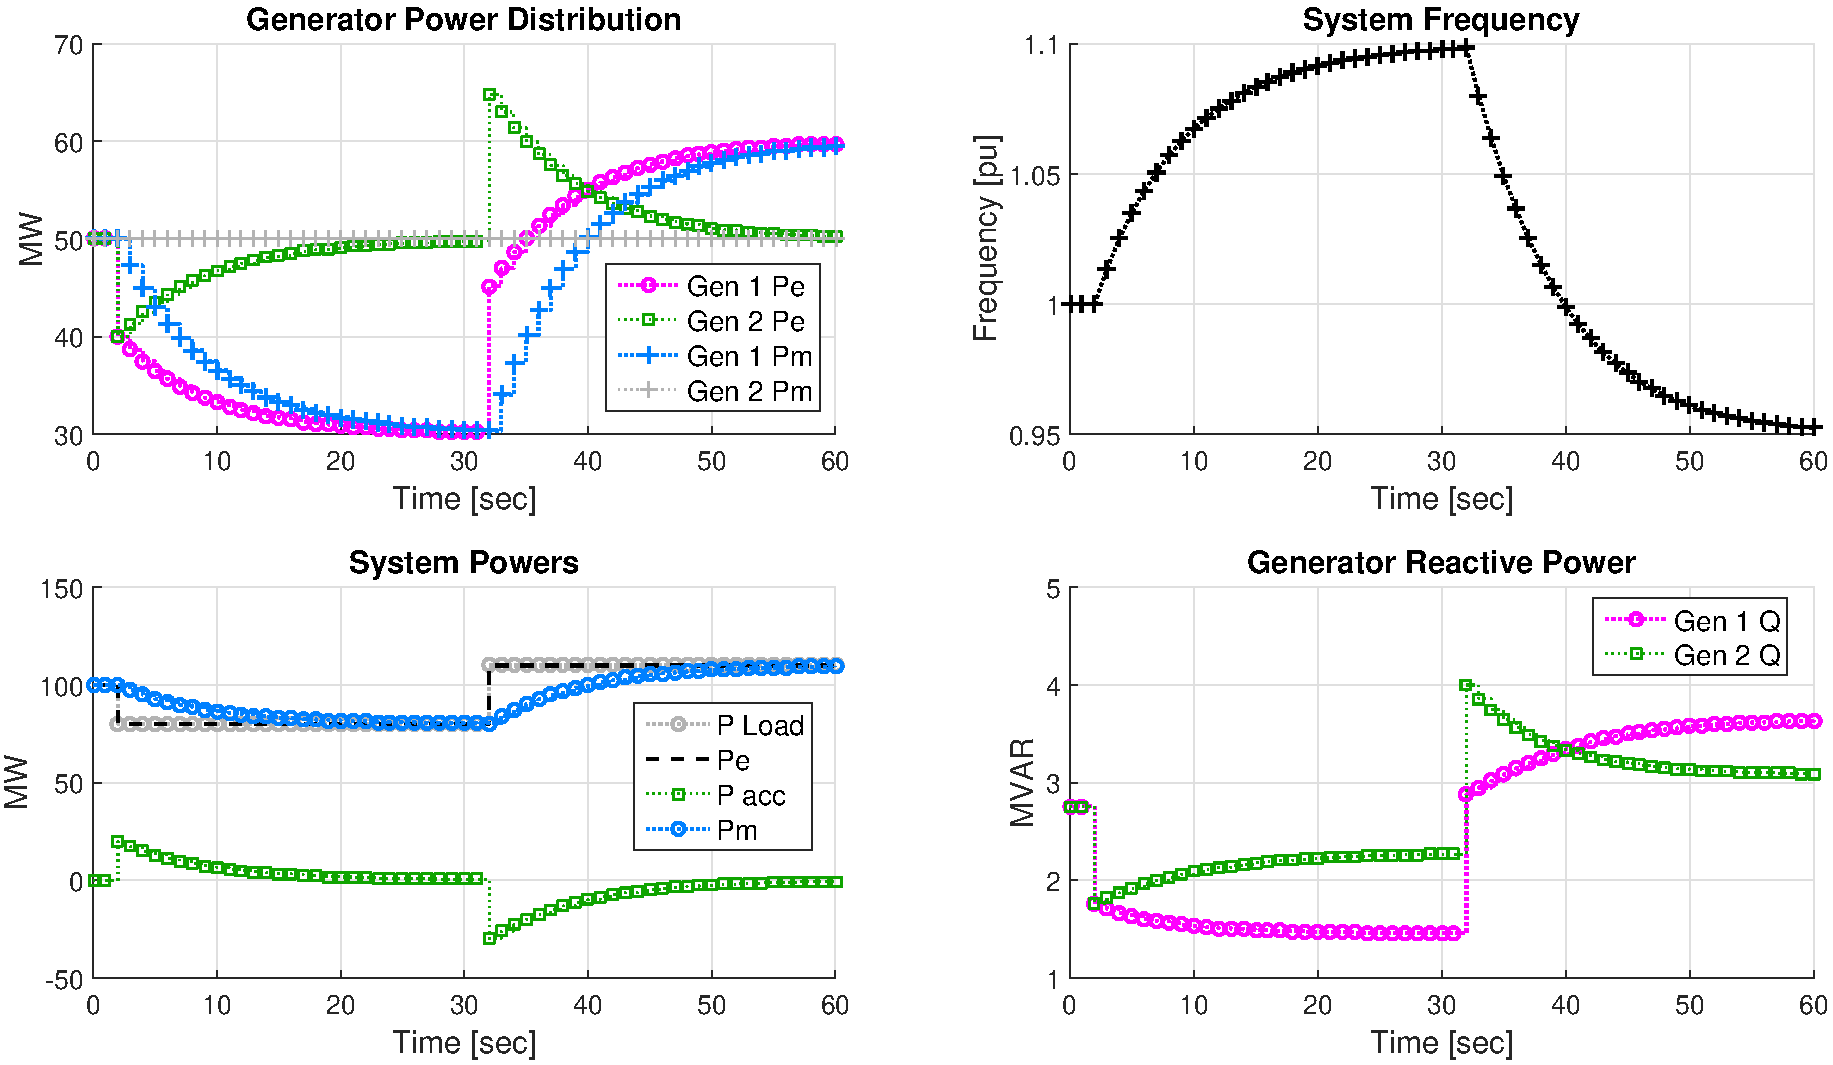
\includegraphics[width=\linewidth]{pgov1x1.pdf}
\end{figure}
\end{frame}
%------------------------------------------------
\begin{frame}
pgov1 on Gen 1 \& Gen 2
\begin{figure}
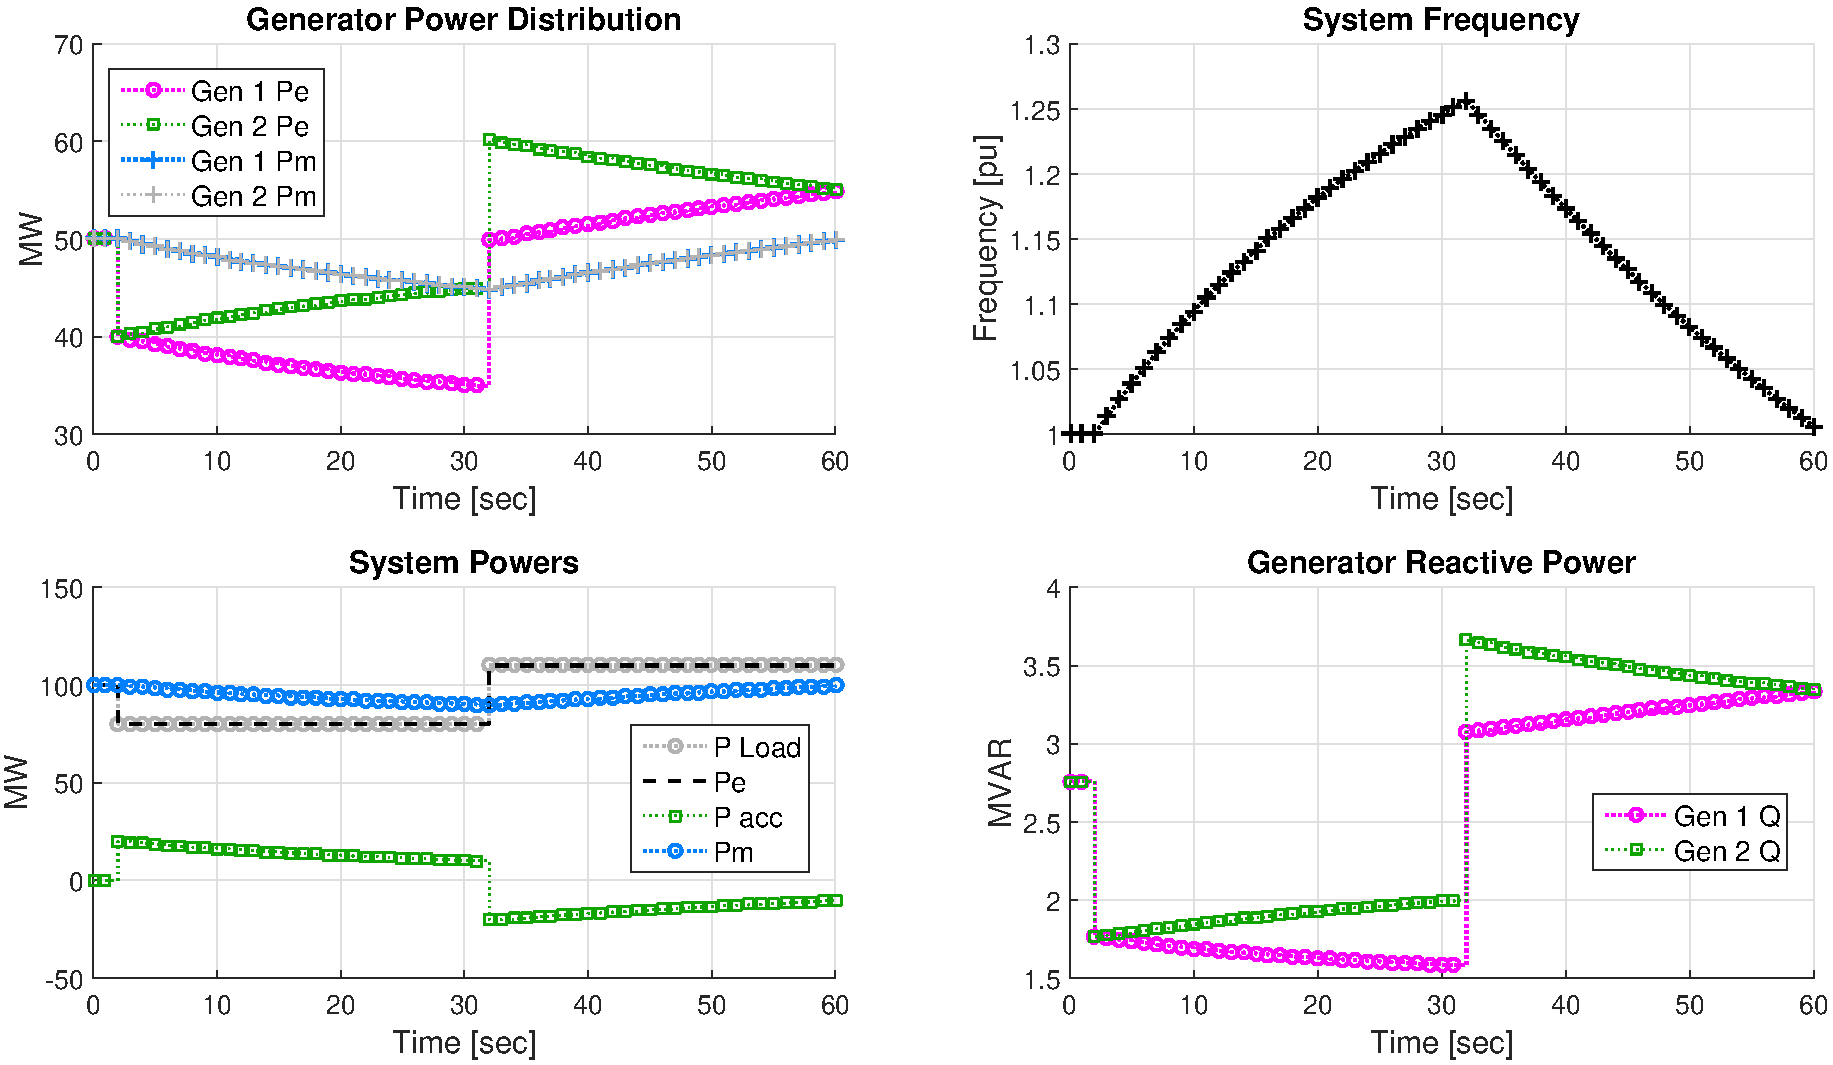
\includegraphics[width=\linewidth]{pgov1x2.pdf}
\end{figure}
\end{frame}


%************************************************
\section{Current Conclusions}
%------------------------------------------------
\begin{frame}
\begin{itemize}
	\item Much more work to do.
	\item Frequency effects should be accounted for in swing equation.
	\item Euler Integration tracks PSLF mean frequency well.
	\item Custom dynamic model implementation seems realizable. 
\end{itemize}
\end{frame}
%------------------------------------------------
\begin{comment}
\subsection{References}
\begin{frame}
\resizebox{.8\textwidth}{.4\textheight}{
\begin{minipage}{\textwidth}
	\begin{itemize}
	\item[[1]] https://spectrum.ieee.org/energy/policy/rebuilding-puerto-ricos-power-grid-the-inside-story
	\item[[2]] https://www.economist.com/united-states/2017/10/19/the-story-of-puerto-ricos-power-grid-is-the-story-of-puerto-rico
	\item[[3]] https://twitter.com/AEEONLINE/status/1006493557908279297/photo/1
	\item[[4]] https://www.nytimes.com/2018/08/14/us/puerto-rico-electricity-power.html
\end{itemize}
\end{minipage}
}
\end{frame}
\end{comment}
\end{document}